\chapter{总体设计}
\section{软件描述}
系统包括服务器端、用户端和开发者端三个部分。

服务器端主要功能是:维护应用、开发者、用户的数据,响应和处理开发者端、用户端的请求,
提供管理人员管理接口,便于维护更新与第三方的接入。

用户端主要功能是:支持用户查询、下载、更新、安装、删除应用,并且能够对应用评价、评分。

开发者端端主要功能是:支持开发者上传、更新、删除应用,并且能够查询收入、将收入提现或转账、查询或回复应用的评价。

\section{处理流程}
\subsection{总体流程}
%overall_overall.png
\begin{figure}[ht]
	\centering
	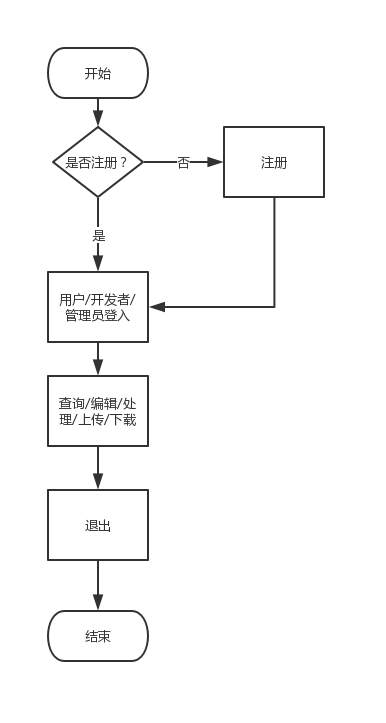
\includegraphics[width=8cm]{overall_overall.png}
	\caption{总体流程} \label{fig:overall_overall.png}
\end{figure}

总体流程针对使用者的逻辑。见图\ref{fig:overall_overall.png}

无论是开发者、用户还是管理员,都需要都账户,作为账户以及提供权限。

其中管理员的注册需要额外的信息以及身份验证。

\subsection{系统基本流程}
%overall_system.png
\begin{figure}[ht]
	\centering
	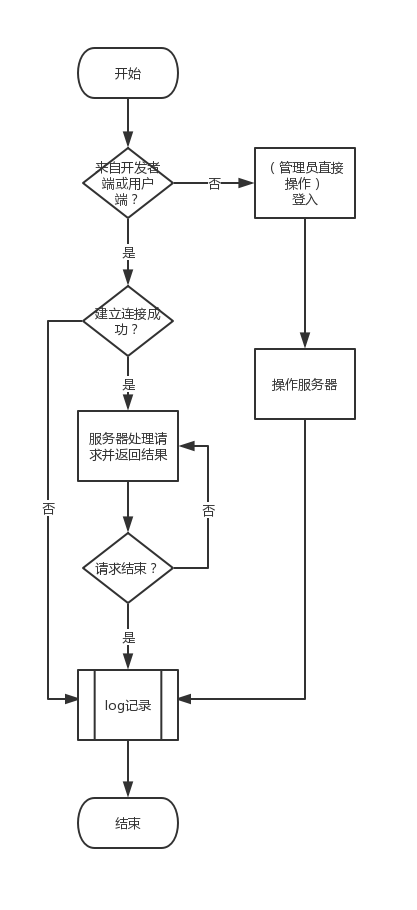
\includegraphics[width=10cm]{overall_system.png}
	\caption{系统基本流程} \label{fig:overall_system.png}
\end{figure}

系统基本流程简要表述不同的端与服务器的交互逻辑,见图\ref{fig:overall_system.png}.

主要需要区分管理人员和普通用户(包括应用开发人员)

普通用户是通过开发者端或者用户段软件与服务器进行连接,
然后请求通过网络交由服务器处理;而管理员需要使用另外的专门的接口,通过命令来操作。

\subsection{客户端基本流程}

我们之前提到过,不对开发者和普通用户用户作严格区分,两者共用一个客户端,开发者一定是普通用户,但反过来不成立。
\begin{figure}[ht]
	\centering
	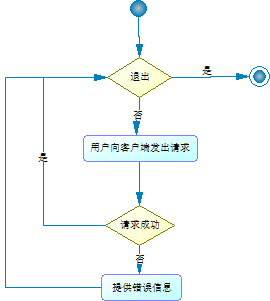
\includegraphics[width=6cm]{overall_client.png}
	\caption{客户端基本流程} \label{fig:overall_client.png}
\end{figure}
简单描述客户端处理用户请求的逻辑,见图\ref{fig:overall_client.png}

\subsection{客户端.注册与登录请求处理功能}
\begin{figure}[ht]
	\centering
	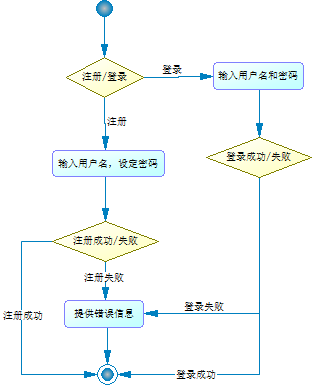
\includegraphics[width=10cm]{client_reg_login.png}
	\caption{客户端.注册与登录请求处理具体流程} \label{fig:client_reg_login.png}
\end{figure}

对于客户的登录与注册请求,见图\ref{fig:client_reg_login.png}

\subsection{客户端.普通用户应用管理请求处理功能}
\begin{figure}[ht]
	\centering
	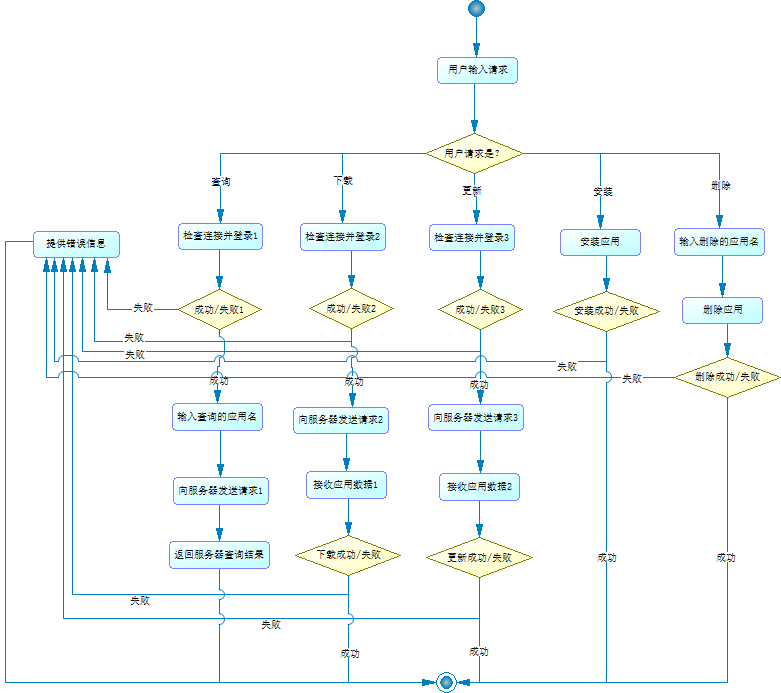
\includegraphics[width=16cm]{client_app.png}
	\caption{客户端.普通用户应用管理请求处理具体流程} \label{fig:client_app.png}
\end{figure}

对于客户的应用管理请求,见图\ref{fig:client_app.png}

\subsection{客户端.普通用户信息反馈请求处理功能}
\begin{figure}[ht]
	\centering
	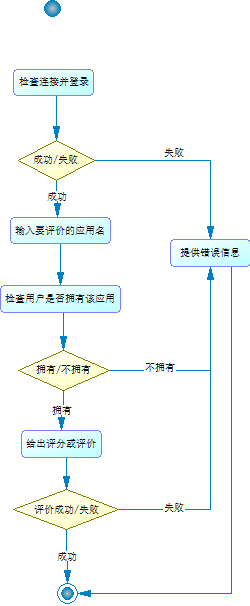
\includegraphics[width=8cm]{client_info.png}
	\caption{客户端.普通用户信息反馈处理具体流程} \label{fig:client_info.png}
\end{figure}

对于客户的信息反馈请求,见图\ref{fig:client_info.png}

\subsection{客户端.开发者应用管理请求处理功能}
\begin{figure}[ht]
	\centering
	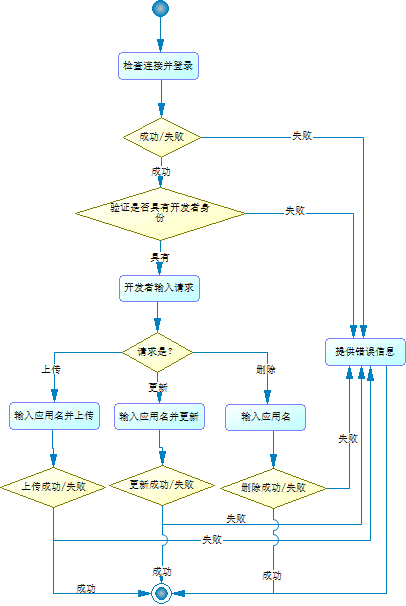
\includegraphics[width=10cm]{developer_app.png}
	\caption{客户端.开发者应用管理请求处理具体流程} \label{fig:developer_app.png}
\end{figure}

对于开发者的应用管理请求,见图\ref{fig:developer_app.png}

\subsection{客户端.开发者信息反馈请求处理功能}
\begin{figure}[ht]
	\centering
	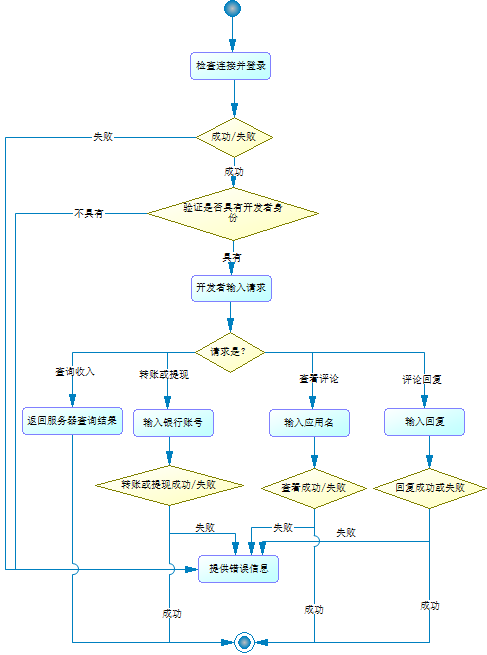
\includegraphics[width=12cm]{developer_info.png}
	\caption{客户端.开发者信息反馈请求处理具体流程} \label{fig:developer_info.png}
\end{figure}

对于开发者的信息反馈请求,见图\ref{fig:developer_info.png}


\subsection{服务器端基本流程}
%overall_sys.png
\begin{figure}[ht]
	\centering
	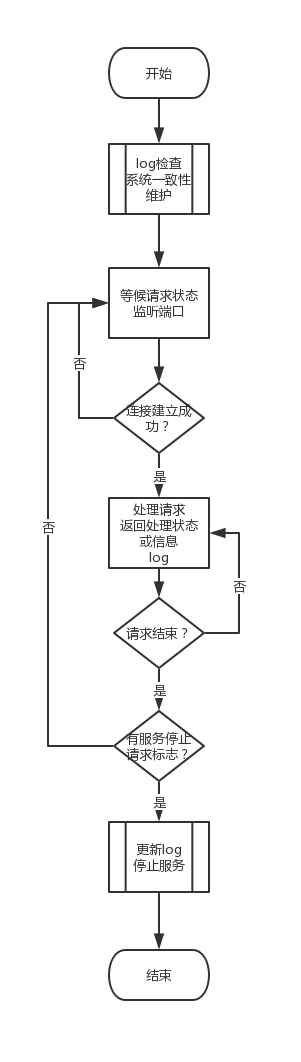
\includegraphics[width=6cm]{overall_sys.png}
	\caption{服务器端基本流程} \label{fig:overall_sys.png}
\end{figure}
简单描述服务器端处理请求的逻辑,见图\ref{fig:overall_sys.png}    .
注意管理员与服务器的交互也是通过网络连接的。
但是管理员没有相应的UI界面。


\subsection{服务器.注册与登录请求处理具体流程}
%overall_sys_login.png
\begin{figure}[ht]
	\centering
	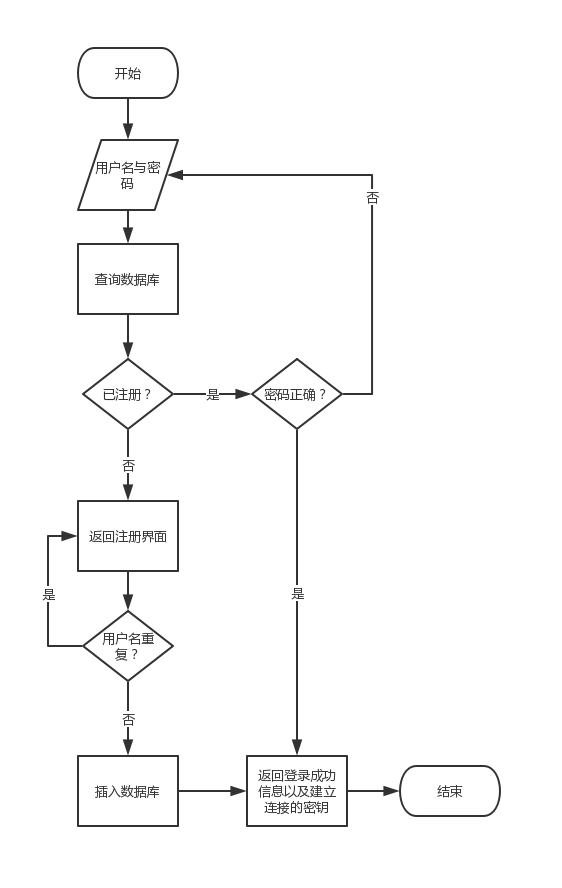
\includegraphics[width=12cm]{overall_sys_login.png}
	\caption{服务器.注册与登录请求处理具体流程} \label{fig:overall_sys_login.png}
\end{figure}

对于2类人员的登录与注册处理,见图\ref{fig:overall_sys_login.png}

此处的注册不包括管理员的注册,因为管理员的注册需要更多的权限,需要通过其他管理员添加进注册人员
列表。

\subsection{服务器.信息查询与修改请求处理具体流程}
%overall_sys_info.png
\begin{figure}[ht]
	\centering
	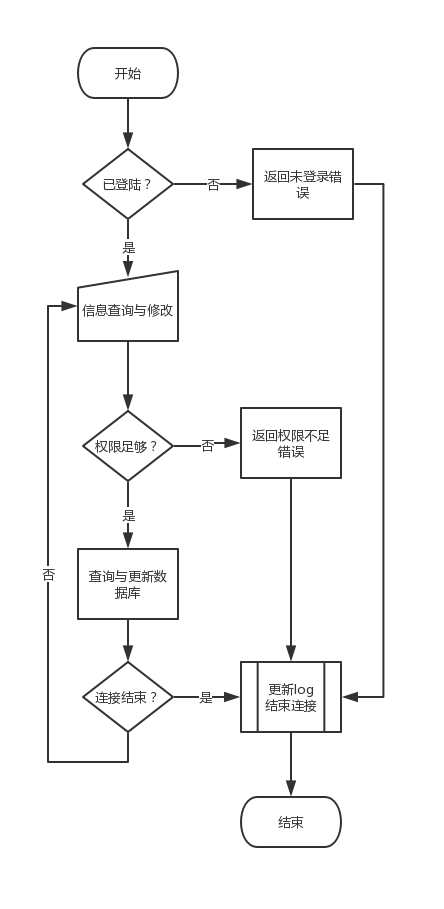
\includegraphics[width=10cm]{overall_sys_info.png}
	\caption{服务器.信息查询与修改请求处理具体流程} \label{fig:overall_sys_info.png}
\end{figure}

对于3类人员的信息查询与修改处理,见图\ref{fig:overall_sys_info.png}

修改需要额外的权限,比如非本app的开发人员不能修改该app的名称,简介等等。

\subsection{服务器.应用上传与下载请求处理具体流程}
%overall_sys_app.png
\begin{figure}[ht]
	\centering
	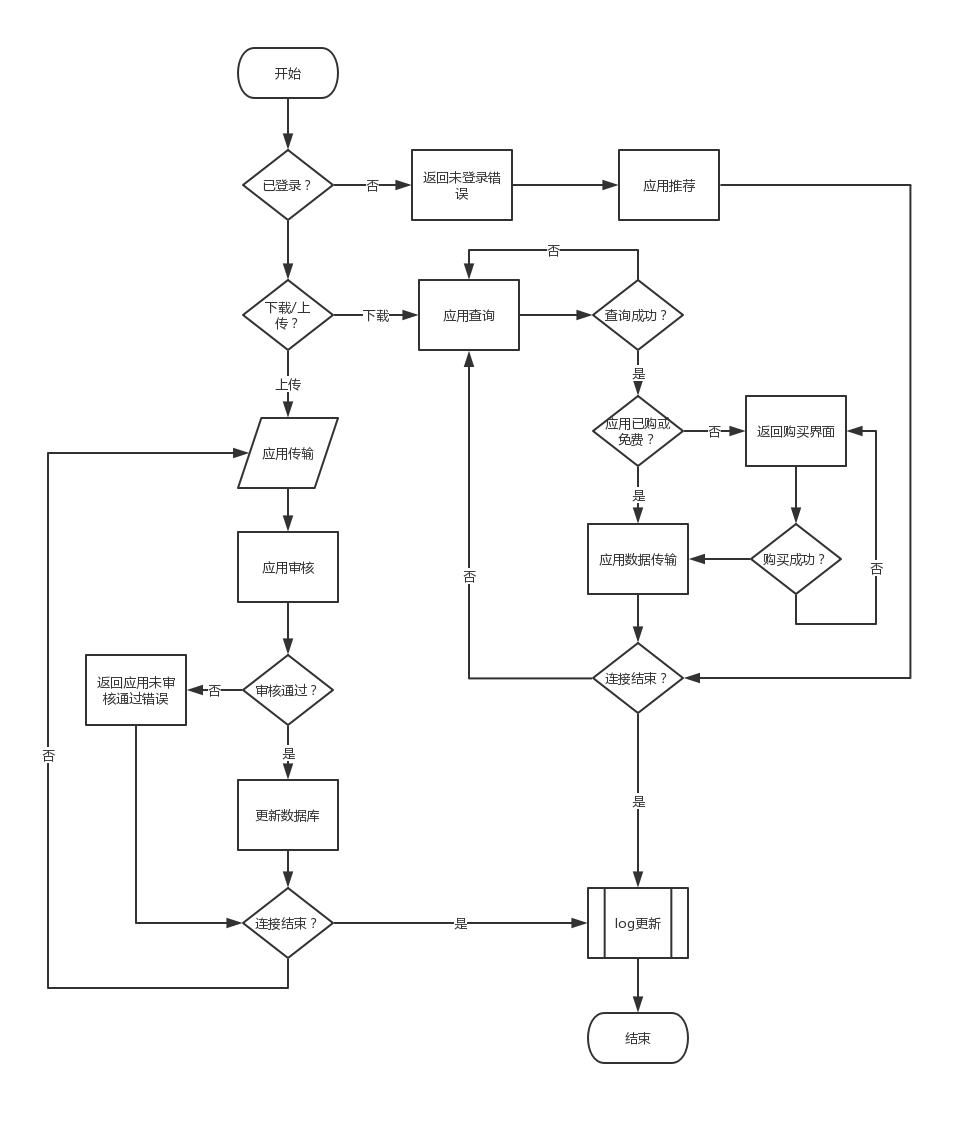
\includegraphics[width=16cm]{overall_sys_app.png}
	\caption{服务器.应用上传与下载请求处理具体流程} \label{fig:overall_sys_app.png}
\end{figure}

对于应用的上传与下载处理见图\ref{fig:overall_sys_app.png}.

上传有应用审核的要求,此处没有具体实现,同时搜索界面也有根据用户的习惯或者统计数据的
自动推荐功能。

\subsection{服务器.账户充值与提现请求处理具体流程}
%overall_sys_account.png
\begin{figure}[ht]
	\centering
	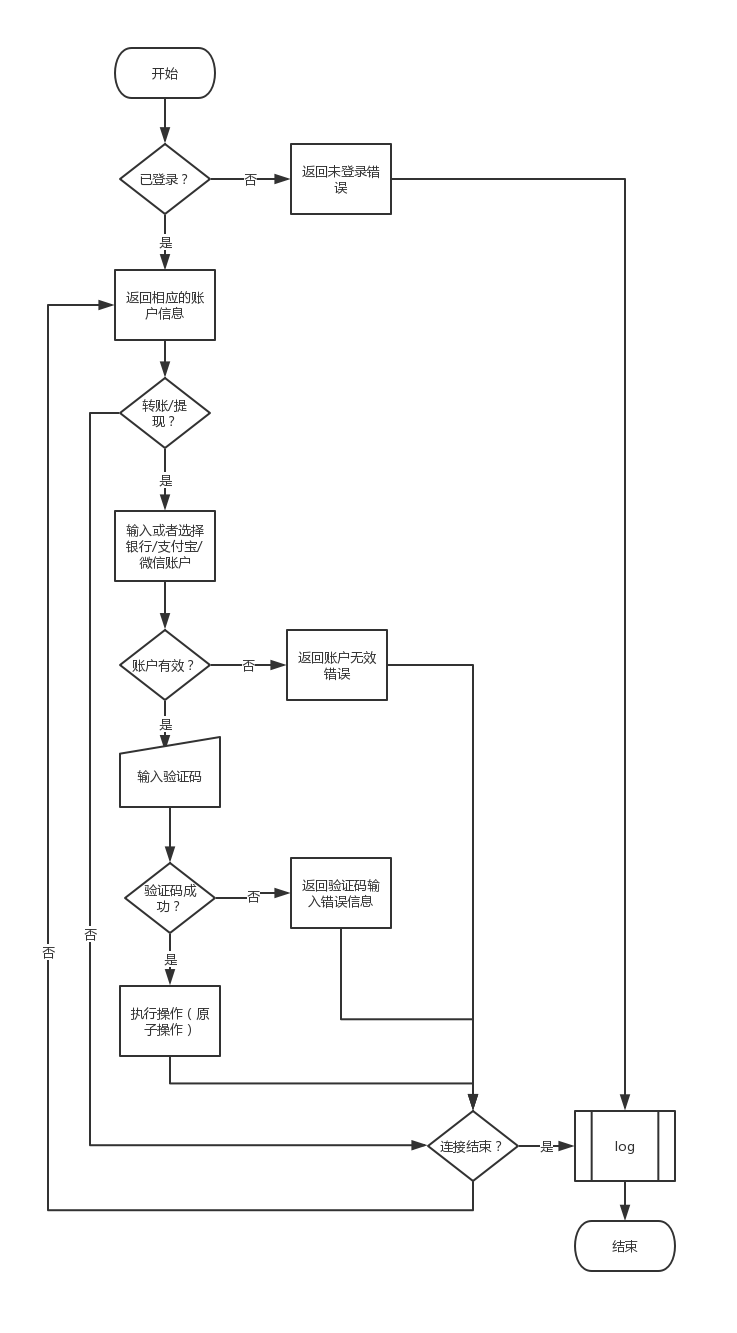
\includegraphics[width=13cm]{overall_sys_account.png}
	\caption{服务器.账户充值与提现请求处理具体流程} \label{fig:overall_sys_account.png}
\end{figure}

对于账户的管理见图\ref{fig:overall_sys_account.png}

可以添加不同的账户,这一点需要在后面提供统一的对外接口。

\subsection{服务器.应用信息查询与更新请求处理具体流程}
%overall_sys_app_info.png
\begin{figure}[ht]
	\centering
	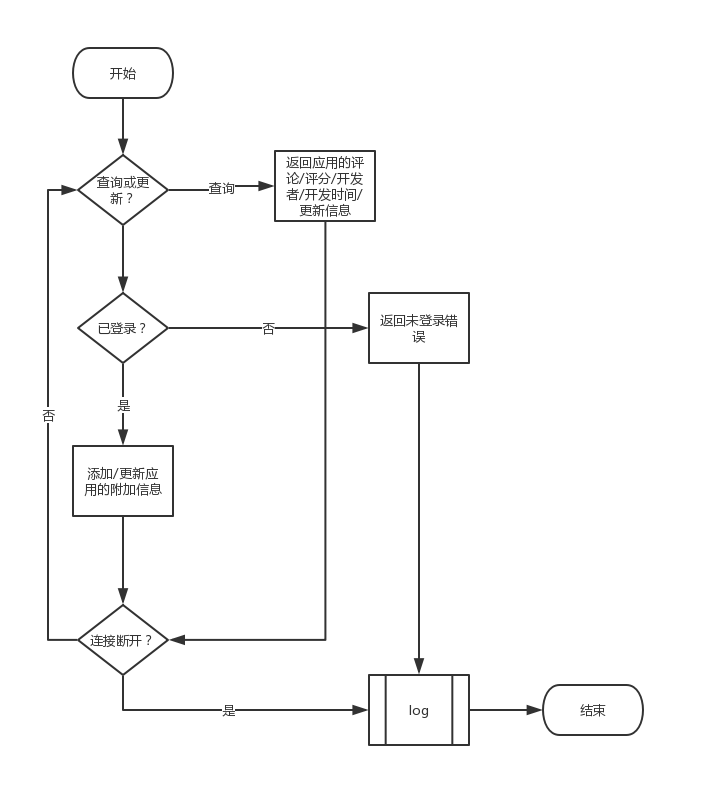
\includegraphics[width=14cm]{overall_sys_app_info.png}
	\caption{服务器.应用信息查询与更新请求处理具体流程} \label{fig:overall_sys_app_info.png}
\end{figure}

对应用的信息查询与评价、评分流程见\ref{fig:overall_sys_app_info.png}.

应用的信息主要针对某个app的评论与评分等等基本信息,与个人信息区分开。

\subsection{服务器.管理员操作请求处理具体流程}
%overall_sys_admin.png
\begin{figure}[ht]
	\centering
	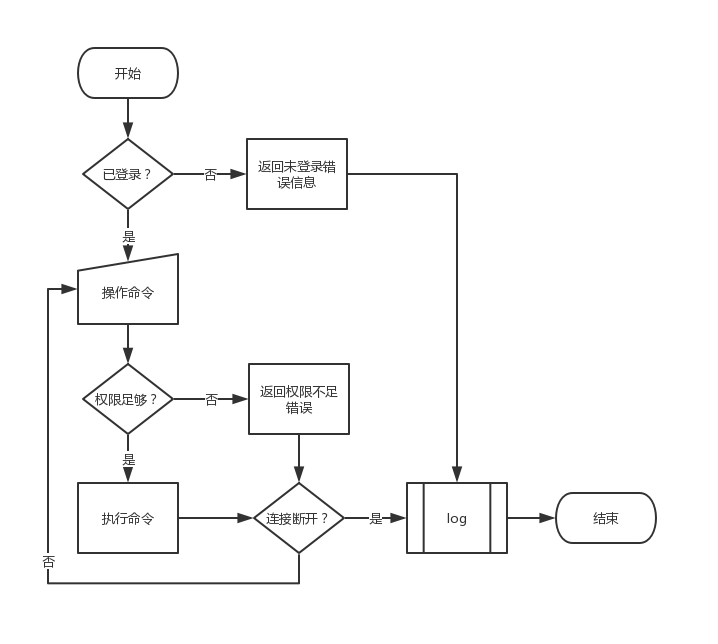
\includegraphics[width=14cm]{overall_sys_admin.png}
	\caption{服务器.管理员操作请求处理具体流程} \label{fig:overall_sys_admin.png}
\end{figure}

对于管理员级别的操作,见图\ref{fig:overall_sys_admin.png}

管理员直接通过命令行与服务器建立连接,同时需要检查每项操作的权限。

{\color{red}
\subsection{应用开发系统}
%overall_devsys.png
\begin{figure}[ht]
	\centering
	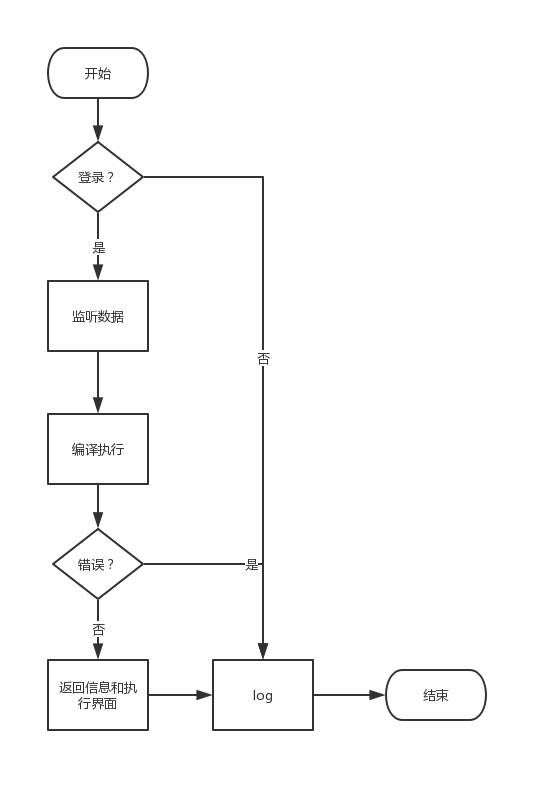
\includegraphics[width=10cm]{overall_devsys.png}
	\caption{服务器.管理员操作请求处理具体流程} \label{fig:overall_devsys.png}
\end{figure}


此处结合开发者端、服务器端、用户端,统一处理流程为图\ref{fig:overall_devsys.png}

}

\section{功能结构设计}
\subsection{整体结构}
%overall_structure0.png
\begin{figure}[ht]
	\centering
	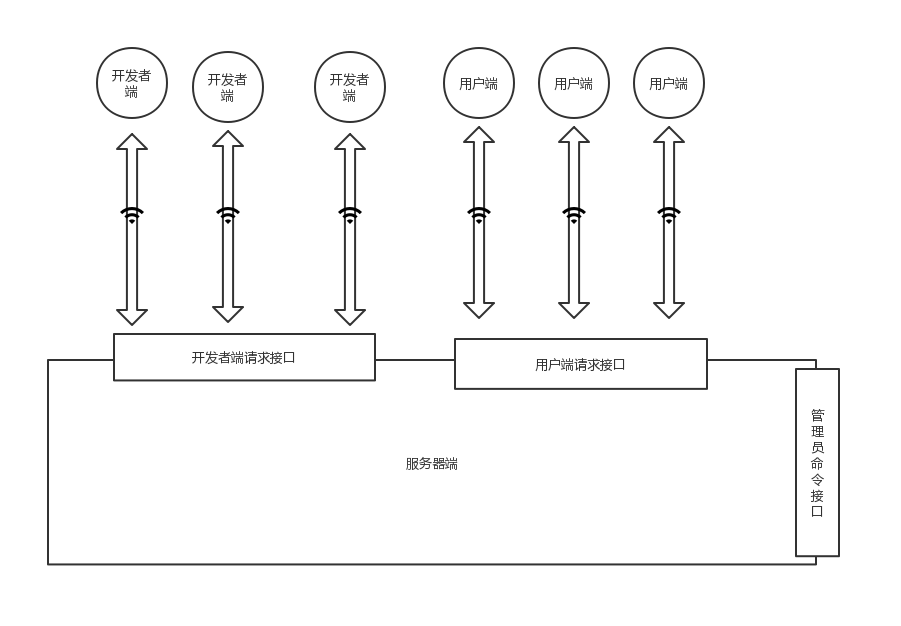
\includegraphics[width=16cm]{overall_structure0.png}
	\caption{整体结构} \label{fig:overall_structure0.png}
\end{figure}

整体结构见图\ref{fig:overall_structure0.png}

服务器端提供3种不同的对外接口,分别针对开发者、用户、管理员。


\subsection{客户端结构}
\begin{figure}[ht]
	\centering
	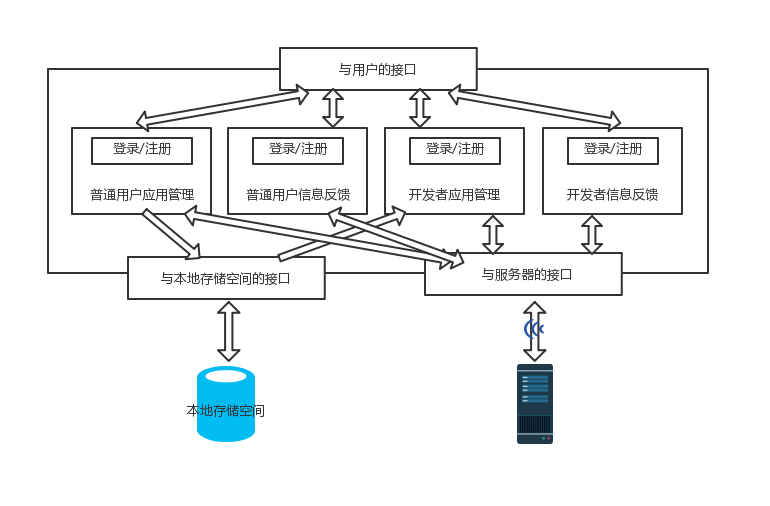
\includegraphics[width=12cm]{client_structure.png}
	\caption{客户端结构} \label{fig:client_structure}
\end{figure}

客户端的结构见图\ref{fig:client_structure}。

注意到,客户端可分为5个模块,其中注册/登录模块只会在其他模块中被调用,其他的模块相互独立。

\subsection{服务器端结构}
%overall_structure.png
\begin{figure}[ht]
	\centering
	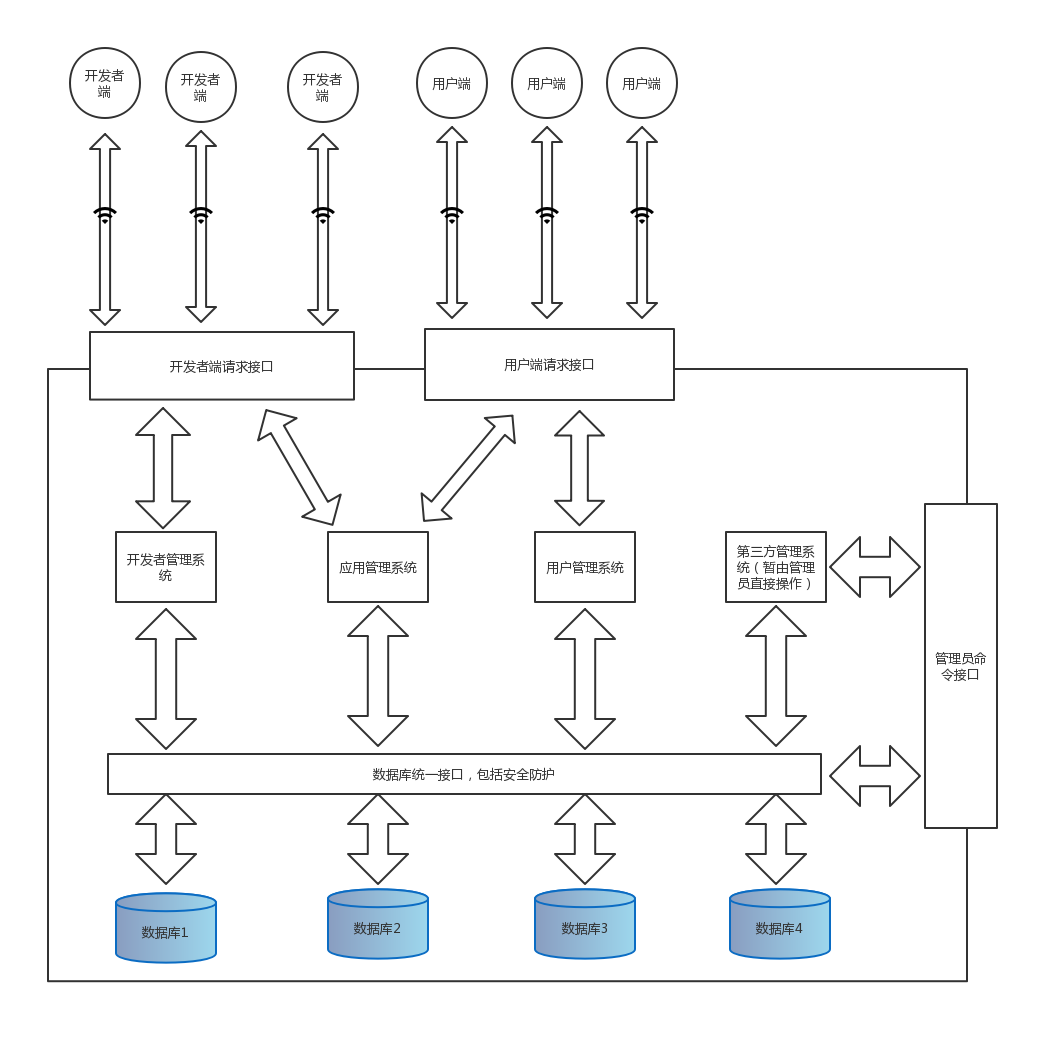
\includegraphics[width=16cm]{overall_structure.png}
	\caption{服务器端结构} \label{fig:overall_structure.png}
\end{figure}

服务器端结构见图\ref{fig:overall_structure.png}

服务器端的内部储存采用数据库,分布且冗余,避免物理失效。

为了安全起见,对外统一有数据库统一接口,接口的修改只能是最高权限的管理员。

普通管理员对外接口也是通过数据库统一接口操作的,同时兼任第三方管理系统的管理员。


\section{功能需求与程序代码的关系}
[此处指的是不同的需求分配到哪些模块去实现。可按不同的端拆分此表]
\begin{table}[htbp]
\centering
\caption{功能需求与程序代码的关系表} \label{tab:requirement-module}
\begin{tabular}{|c|c|c|c|c|c|}
    \hline
    需求编码 & 需求名称 & 开发者端应用管理模块 & 开发者端信息反馈模块 & 客户端应用管理模块 & 客户端信息反馈模块\\
    \hline
    SRS\_Dev\_App\_P01 & 开发者端.应用管理 & Y & · & . & .\\
    \hline
    SRS\_Dev\_Info\_P01 & 开发者端.信息反馈 & . & Y & . & .\\
    \hline
    SRS\_User\_App\_P01 & 客户端.应用管理 & . & · & Y & .\\
    \hline
    SRS\_User\_Info\_P01 & 客户端.信息反馈 & · & · & . & Y\\
    \hline
\end{tabular}
\note{各项功能需求的实现与各个程序模块的分配关系}
\end{table}